\documentclass{article}
\usepackage[UTF8]{ctex}
\usepackage{geometry}
\usepackage{makecell}
\usepackage{amsmath}
\usepackage{graphicx}
\usepackage{subcaption}
\usepackage{bigstrut}

\geometry{a4paper,scale=0.75}

\title{\heiti 实验十八\ 弗兰克-赫兹实验}
\author{\kaishu 田睿轩\ 物理学院\ 1900011602}
\date{2020年12月12日}
\newcommand{\degree}{^\circ}
\newcommand{\degreesCelsius}{^\circ C}

\begin{document}
    \maketitle
    \section{数据处理}
    \subsection{弗兰克-赫兹管的扫描结果}
    \subsubsection{Hg管}
    实验中使用四栅式弗兰克-赫兹管,实验装置如图所示:\par
    \begin{center}
        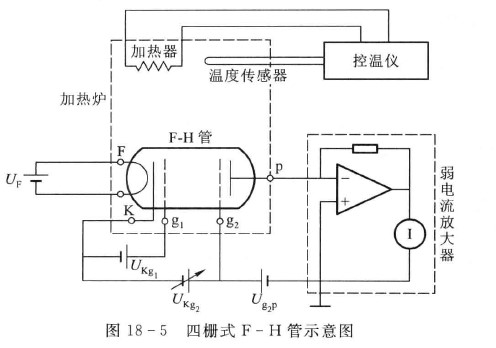
\includegraphics[width=0.5\textwidth]{experiment utility.jpg}
    \end{center}

    装置中,F-H管中充汞蒸气或氩气,$U_1(U_{Kg_1})$用于消除灯丝附近的电荷聚集,$U_2(U_{Kg_2})$为加速电压,用来加速灯丝发出的电子,其电压值可
    近似视为电子的最大动能,$U_{g_2P}$为减速电压,电压低于该值的电子无法到达P极,高于该值的电子到达P极并产生电流。
    当加速电压达到汞原子的某激发电压时,电子与汞原子发生非弹性碰撞,汞原子发出光子,电子动能减小,无法经过$U_{g_2P}$到达P极,
    因此电流会发生突降,实验中,通过研究加速电压与P极电流的关系即可研究汞原子或氩原子的激发能级。
    实验中,P极电流通过接在外侧的弱电流放大器两端电压来反映

    本实验中,汞蒸气温度$\theta=175\degreesCelsius$,$U_{Kg_1}=1.05V$,$U_{g_2P}=1.56V$,实验数据如下所示:

    \begin{center}
        \begin{tabular}{|c|c|c|c|c|c|c|c|c|c|c|c|}
            \hline
            $U_2(V)$ & 0.0   & 0.4   & 0.8   & 1.1   & 1.3   & 1.6   & 2.0   & 2.3   & 2.6   & 2.9   & 3.3  \\
            \hline
            $U_0(mV)$ & 8.8   & 9.0   & 9.2   & 9.3   & 9.4   & 9.6   & 9.7   & 9.8   & 9.9   & 10.1  & 11.2  \\
            \hline
        \end{tabular}%           
    \end{center}

    续表

    \begin{center}
        \begin{tabular}{|c|c|c|c|c|c|c|c|c|c|c|c|}
            \hline
            $U_2(V)$ & 3.6   & 3.9   & 4.1   & 4.3   & 4.5   & 4.7   & 4.8   & 4.9   & 5.0   & 5.1   & 5.2 \\
            \hline
            $U_0(mV)$ & 13.0  & 14.2  & 15.2  & 17.3  & 20.1  & 23.0  & 25.8  & 28.0  & 30.5  & 31.8  & 33.8 \\
            \hline
        \end{tabular}%            
    \end{center}

    续表

    \begin{center}
        \begin{tabular}{|c|c|c|c|c|c|c|c|c|c|c|c|}
            \hline
            $U_2(V)$ & 5.3   & 5.4   & 5.5   & 5.8   & 6.2   & 6.5   & 6.8   & 6.9   & 7.1   & 7.3   & 7.6 \\
            \hline
            $U_0(mV)$ & 33.3  & 30.2  & 27.2  & 17.6  & 12.2  & 10.9  & 10.8  & 11.1  & 12.2  & 13.5  & 18.0 \\
            \hline
        \end{tabular}%                    
    \end{center}

    续表

    \begin{center}
        \begin{tabular}{|c|c|c|c|c|c|c|c|c|c|c|c|}
            \hline
            $U_2(V)$ & 7.8   & 8.1   & 8.4   & 8.7   & 9.0   & 9.2   & 9.4   & 9.6   & 9.8   & 9.9   & 10.1 \\
            \hline
            $U_0(mV)$ & 20.4  & 24.3  & 31.4  & 41.4  & 54.1  & 59.8  & 69.4  & 75.5  & 79.0  & 78.2  & 69.5 \\
            \hline
        \end{tabular}%                   
    \end{center}

    续表

    \begin{center}
        \begin{tabular}{|c|c|c|c|c|c|c|c|c|c|c|c|}
            \hline
            $U_2(V)$ & 10.3  & 10.6  & 10.9  & 11.1  & 11.2  & 11.3  & 11.4  & 11.6  & 11.9  & 12.2  & 12.5  \bigstrut\\
            \hline
            $U_0(mV)$ & 46.0  & 19.8  & 15.0  & 12.4  & 11.8  & 11.4  & 11.8  & 12.5  & 15.0  & 20.0  & 23.6  \bigstrut\\
            \hline
        \end{tabular}%                 
    \end{center}

    续表

    \begin{center}
        \begin{tabular}{|c|c|c|c|c|c|c|c|c|c|c|c|}
            \hline
            $U_2(V)$ & 12.8  & 13.1  & 13.4  & 13.7  & 13.9  & 14.1  & 14.3  & 14.5  & 14.6  & 14.8  & 15.0  \bigstrut\\
            \hline
            $U_0(mV)$ & 33.2  & 39.9  & 56.8  & 69.8  & 80.5  & 92.8  & 105.9  & 115.7  & 111.9  & 104.6  & 82.4  \bigstrut\\
            \hline
        \end{tabular}%                           
    \end{center}

    续表

    \begin{center}
        \begin{tabular}{|c|c|c|c|c|c|c|c|c|c|c|c|}
            \hline
            $U_2(V)$ & 15.2  & 15.5  & 15.8  & 16.0  & 16.2  & 16.3  & 16.5  & 16.8  & 17.1  & 17.4  & 17.7  \bigstrut\\
            \hline
            $U_0(mV)$ & 47.8  & 27.6  & 18.2  & 14.1  & 13.6  & 13.2  & 14.8  & 18.9  & 22.3  & 31.6  & 38.2  \bigstrut\\
            \hline
        \end{tabular}%                                     
    \end{center}

    续表

    \begin{center}
        \begin{tabular}{|c|c|c|c|c|c|c|c|c|c|c|c|}
            \hline
            $U_2(V)$ & 17.9  & 18.3  & 18.6  & 18.9  & 19.1  & 19.3  & 19.4  & 19.6  & 19.8  & 20.1  & 20.4  \bigstrut\\
            \hline
            $U_0(mV)$ & 47.5  & 66.6  & 94.9  & 123.9  & 147.6  & 165.2  & 158.5  & 153.8  & 132.0  & 90.8  & 53.7  \bigstrut\\
            \hline
        \end{tabular}%                                                
    \end{center}

    续表

    \begin{center}
        \begin{tabular}{|c|c|c|c|c|c|c|c|c|c|c|c|}
            \hline
            $U_2(V)$ & 20.6  & 20.8  & 21.0  & 21.0  & 21.4  & 21.6  & 21.9  & 22.2  & 22.5  & 22.8  & 23.2  \bigstrut\\
            \hline
            $U_0(mV)$ & 42.0  & 27.3  & 23.8  & 19.6  & 19.5  & 21.0  & 25.3  & 36.8  & 48.6  & 62.9  & 97.1  \bigstrut\\
            \hline
        \end{tabular}%                                                         
    \end{center}

    续表

    \begin{center}
        \begin{tabular}{|c|c|c|c|c|c|c|c|c|c|c|c|}
            \hline
            $U_2(V)$ & 23.5  & 23.8  & 24.0  & 24.2  & 24.3  & 24.5  & 24.7  & 25.0  & 25.3  & 25.5  & 25.7  \bigstrut\\
            \hline
            $U_0(mV)$ & 113.8  & 152.6  & 176.6  & 187.9  & 185.8  & 182.8  & 151.9  & 120.0  & 81.7  & 60.3  & 45.6  \bigstrut\\
            \hline
        \end{tabular}%                                                                 
    \end{center}

    续表

    \begin{center}
        \begin{tabular}{|c|c|c|c|c|c|c|c|c|c|c|c|}
            \hline
            $U_2(V)$ & 25.9  & 26.1  & 26.3  & 26.5  & 26.8  & 27.0  & 27.3  & 27.7  & 28.0  & 28.3  & 28.6  \bigstrut\\
            \hline
            $U_0(mV)$ & 35.1  & 30.1  & 28.8  & 29.1  & 33.0  & 39.9  & 47.3  & 70.5  & 96.1  & 130.6  & 148.9  \bigstrut\\
            \hline
        \end{tabular}%                                                                            
    \end{center}

    续表

    \begin{center}
        \begin{tabular}{|c|c|c|c|c|c|c|c|c|}
            \hline
            $U_2(V)$ & 28.8  & 29.0  & 29.2  & 29.3  & 29.4  & 29.6  & 29.8  & 30.0  \bigstrut\\
            \hline
            $U_0(mV)$ & 169.9  & 183.9  & 197.7  & 199.2  & 200.5  & 191.9  & 174.0  & 158.0  \bigstrut\\
            \hline
        \end{tabular}%                                                                          
    \end{center}

    将测量所得数据绘制曲线,如下图所示:
    
    \begin{center}
        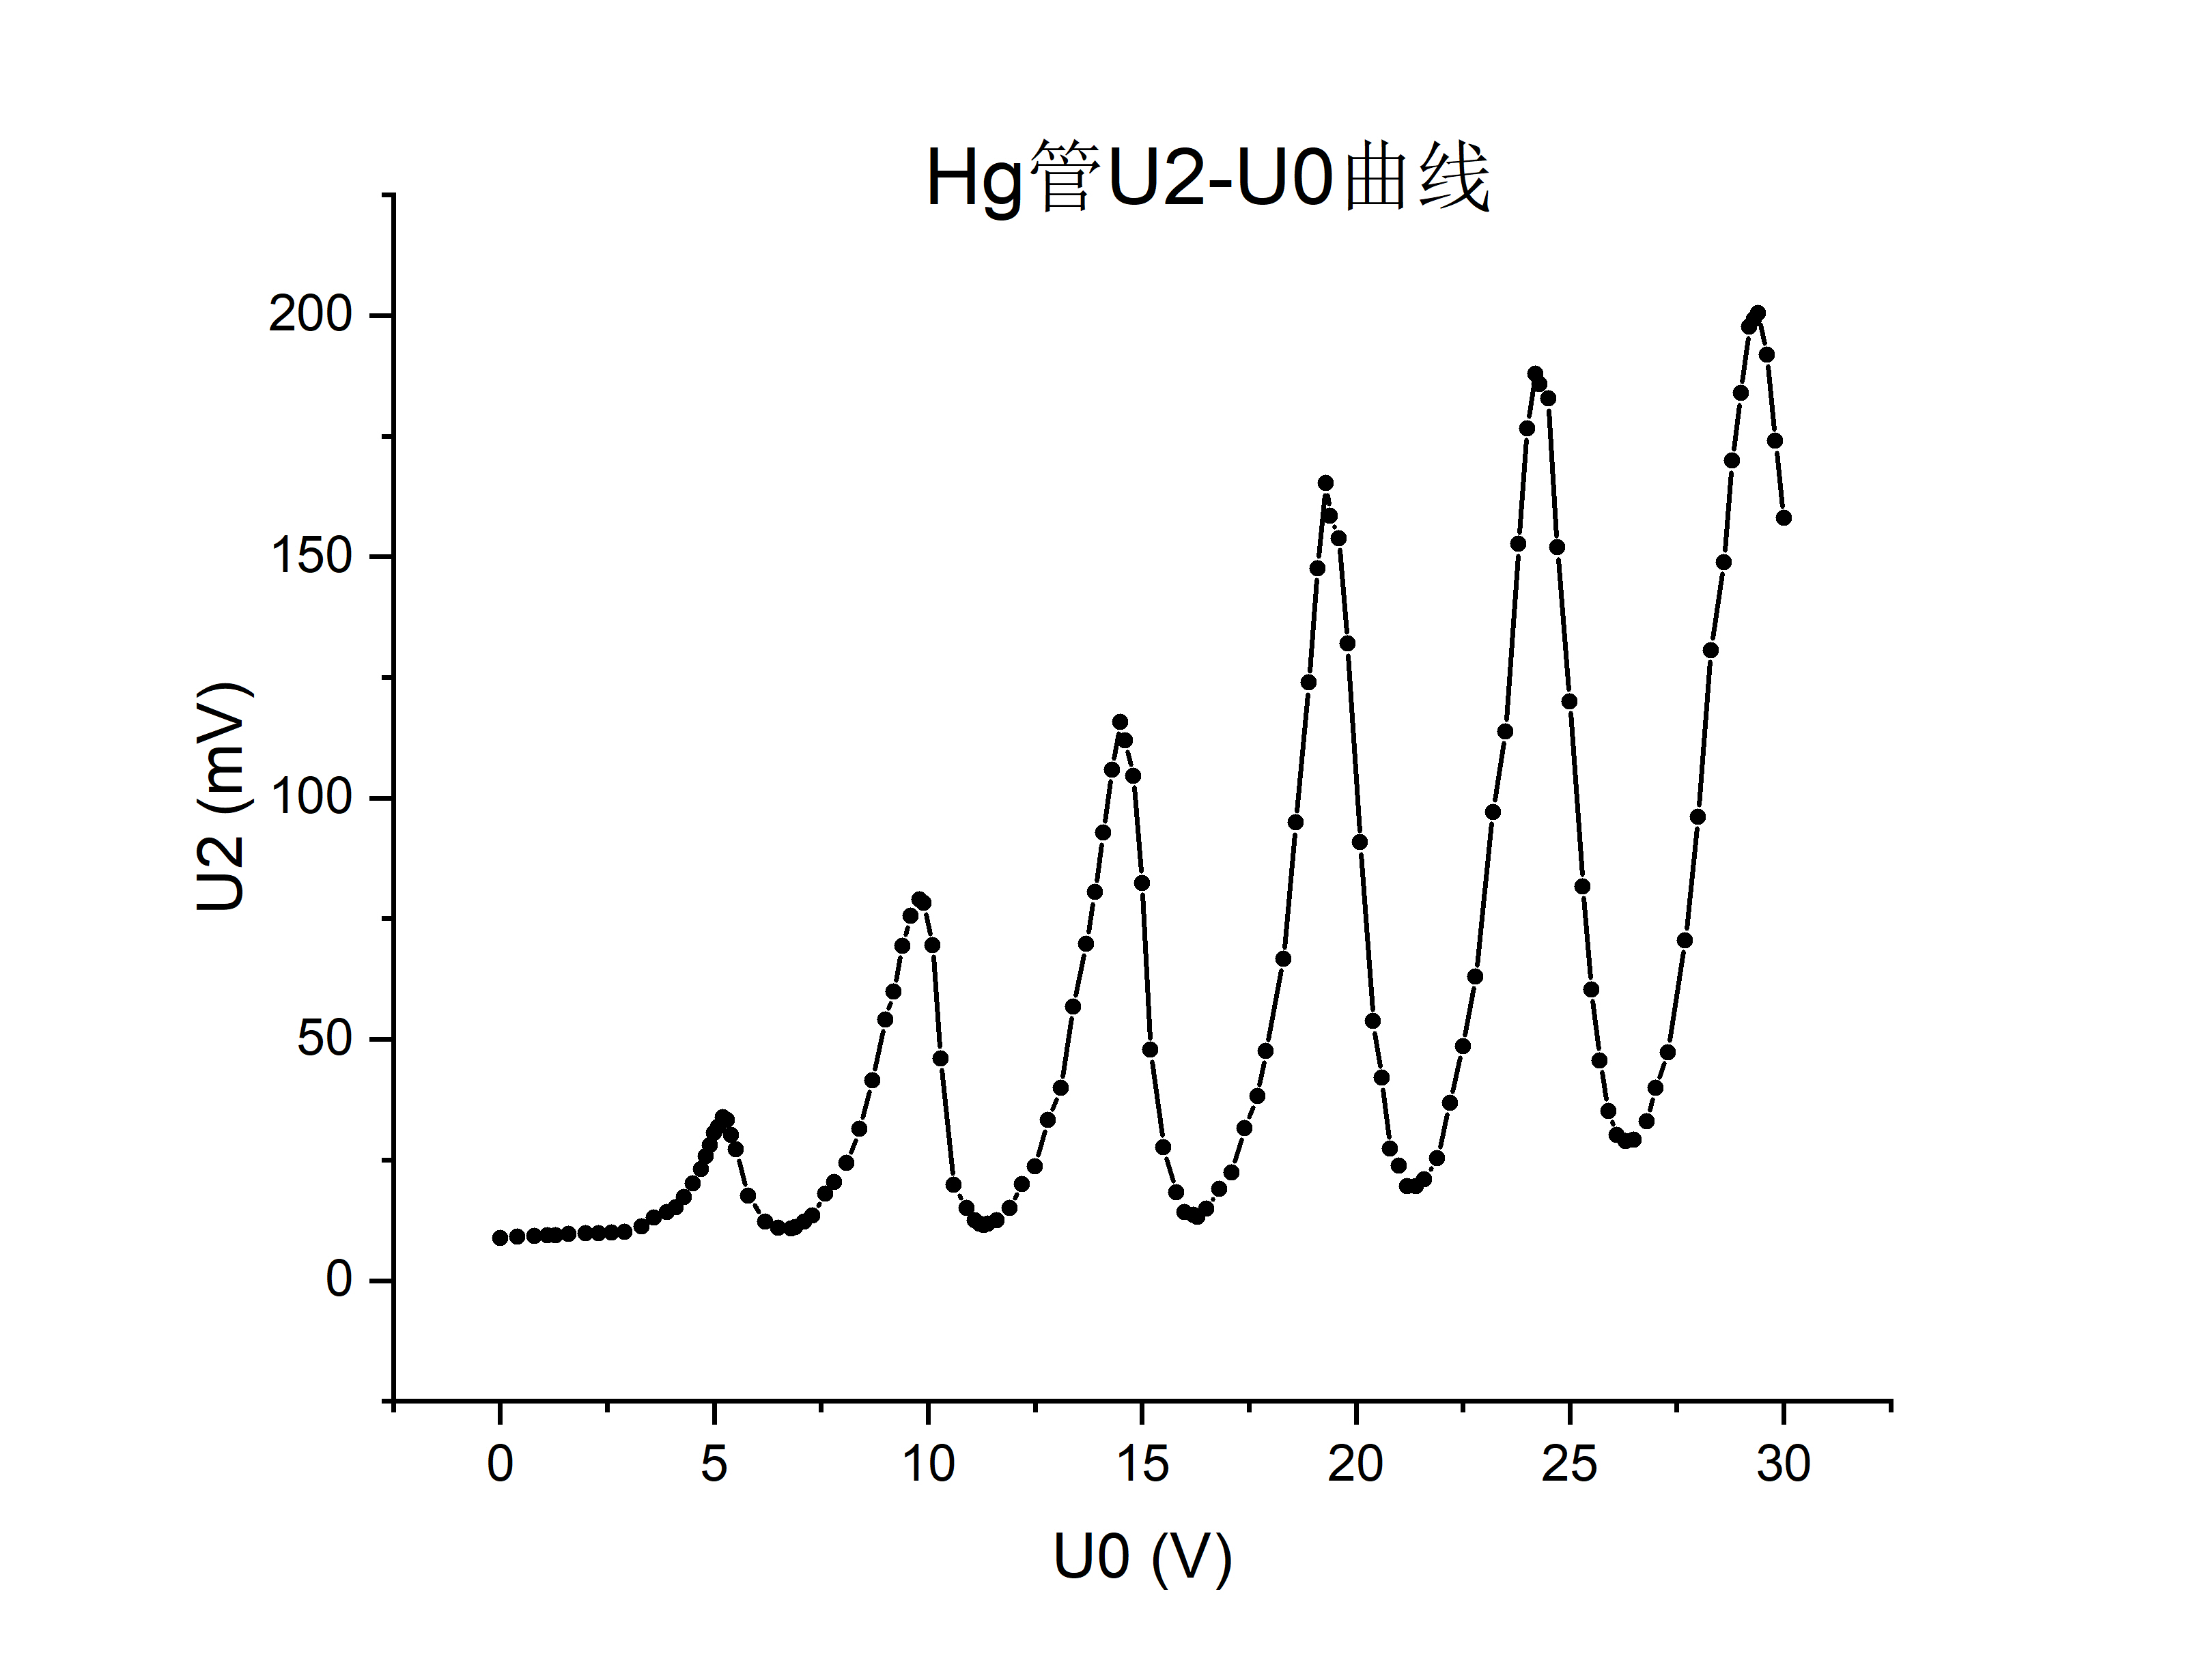
\includegraphics[width=0.8\textwidth]{Hg curve1.jpg}
    \end{center}

    从曲线中,可以看出电压呈现周期性上升和下降,从定型上符合理论的预期。

    \subsubsection{Ar管}
    氩管的实验装置与汞管类似,但由于氩在常温下为气态,故不需要加热。氩管的P极电流由装置直接探测。
    
    实验中,旁热式电极的电压$U_{F}=2.8V$,$U_{Kg_1}=2.0V$,$U_{g2_P}=6.5V$,P极电流的量程选$\times 10(-8)A$。
    实验数据如下表所示:

    \begin{center}
        \begin{tabular}{|c|c|c|c|c|c|c|c|c|c|c|c|}
            \hline
            $U_2(V)$ & 0.0   & 1.0   & 2.0   & 2.5   & 3.0   & 4.0   & 5.0   & 6.0   & 7.0   & 8.0   & 8.4  \bigstrut\\
            \hline
            $I_0(\times 10^{-8}A)$ & 0.0   & 0.0   & 0.0   & 0.0   & 0.0   & 0.0   & 0.0   & 0.0   & 0.0   & 0.0   & 0.0  \bigstrut\\
            \hline
        \end{tabular}%            
    \end{center}

    续表

    \begin{center}
        \begin{tabular}{|c|c|c|c|c|c|c|c|c|c|c|c|}
            \hline
            $U_2(V)$ & 8.8   & 9.2   & 10.0  & 10.4  & 10.8  & 11.2  & 11.6  & 12.0  & 12.5  & 13.0  & 13.4  \bigstrut\\
            \hline
            $I_0(\times 10^{-8}A)$ & 0.0   & 0.0   & 0.1   & 0.2   & 0.3   & 0.5   & 0.7   & 0.9   & 1.2   & 1.7   & 2.1  \bigstrut\\
            \hline
        \end{tabular}%          
    \end{center}

    续表

    \begin{center}
        \begin{tabular}{|c|c|c|c|c|c|c|c|c|c|c|c|}
            \hline
            $U_2(V)$ & 13.8  & 14.2  & 14.6  & 15.1  & 15.3  & 15.5  & 15.8  & 16.0  & 16.3  & 16.6  & 16.8  \bigstrut\\
            \hline
            $I_0(\times 10^{-8}A)$ & 2.9   & 3.7   & 5.0   & 6.1   & 6.3   & 6.5   & 7.2   & 7.3   & 7.6   & 7.9   & 8.1  \bigstrut\\
            \hline
        \end{tabular}%         
    \end{center}

    续表

    \begin{center}
        \begin{tabular}{|c|c|c|c|c|c|c|c|c|c|c|c|}
            \hline
            $U_2(V)$ & 17.1  & 17.3  & 17.7  & 18.0  & 18.3  & 18.7  & 19.1  & 19.5  & 19.9  & 20.4  & 20.8  \bigstrut\\
            \hline
            $I_0(\times 10^{-8}A)$ & 8.2   & 8.3   & 8.4   & 8.2   & 8.1   & 7.7   & 7.0   & 6.1   & 5.3   & 4.0   & 3.1  \bigstrut\\
            \hline
        \end{tabular}%        
    \end{center}
    
    续表

    \begin{center}
        \begin{tabular}{|c|c|c|c|c|c|c|c|c|c|c|c|}
            \hline
            $U_2(V)$ & 21.0  & 21.5  & 21.7  & 22.0  & 22.4  & 22.7  & 23.0  & 23.3  & 23.6  & 24.0  & 24.4  \bigstrut\\
            \hline
            $I_0(\times 10^{-8}A)$ & 2.4   & 1.7   & 1.4   & 1.2   & 1.1   & 1.2   & 1.9   & 3.0   & 5.3   & 9.0   & 11.4  \bigstrut\\
            \hline
        \end{tabular}%        
    \end{center}
        
    续表

    \begin{center}
        \begin{tabular}{|c|c|c|c|c|c|c|c|c|c|c|c|}
            \hline
            $U_2(V)$ & 24.8  & 25.2  & 25.7  & 26.2  & 26.7  & 27.1  & 27.4  & 27.7  & 27.9  & 28.3  & 28.6  \bigstrut\\
            \hline
            $I_0(\times 10^{-8}A)$ & 14.4  & 15.8  & 18.2  & 20.5  & 21.8  & 22.5  & 22.7  & 22.9  & 23.2  & 23.2  & 22.8  \bigstrut\\
            \hline
        \end{tabular}%                   
    \end{center}

    续表

    \begin{center}
        \begin{tabular}{|c|c|c|c|c|c|c|c|c|c|c|c|}
            \hline
            $U_2(V)$ & 29.0  & 29.3  & 29.6  & 29.9  & 30.2  & 30.5  & 30.8  & 31.1  & 31.4  & 31.7  & 32.1  \bigstrut\\
            \hline
            $I_0(\times 10^{-8}A)$ & 22.1  & 21.4  & 20.5  & 18.9  & 17.5  & 15.7  & 13.7  & 11.4  & 8.9   & 7.2   & 4.6  \bigstrut\\
            \hline
        \end{tabular}%                  
    \end{center}
    
    续表

    \begin{center}
        \begin{tabular}{|c|c|c|c|c|c|c|c|c|c|c|c|}
            \hline
            $U_2(V)$ & 32.5  & 32.9  & 33.2  & 33.5  & 33.8  & 34.1  & 34.4  & 34.9  & 35.2  & 35.6  & 35.9  \bigstrut\\
            \hline
            $I_0(\times 10^{-8}A)$ & 2.6   & 1.7   & 1.6   & 2.7   & 4.9   & 8.1   & 11.0  & 16.2  & 18.8  & 21.2  & 23.3  \bigstrut\\
            \hline
        \end{tabular}%                  
    \end{center}

    续表

    \begin{center}
        \begin{tabular}{|c|c|c|c|c|c|c|c|c|c|c|c|}
            \hline
            $U_2(V)$ & 36.3  & 36.6  & 37.0  & 37.3  & 37.6  & 38.0  & 38.3  & 38.6  & 38.8  & 39.0  & 39.2  \bigstrut\\
            \hline
            $I_0(\times 10^{-8}A)$ & 26.4  & 27.0  & 28.3  & 30.3  & 31.3  & 32.3  & 33.3  & 34.2  & 34.7  & 35.1  & 35.5  \bigstrut\\
            \hline
        \end{tabular}%                  
    \end{center}

    续表

    \begin{center}
        \begin{tabular}{|c|c|c|c|c|c|c|c|c|c|c|c|}
            \hline
            $U_2(V)$ & 39.4  & 39.7  & 39.9  & 40.1  & 40.3  & 40.6  & 40.9  & 41.2  & 41.5  & 41.8  & 42.1  \bigstrut\\
            \hline
            $I_0(\times 10^{-8}A)$ & 35.7  & 36.1  & 36.2  & 36.1  & 36.0  & 35.5  & 34.7  & 33.8  & 32.6  & 31.0  & 28.5  \bigstrut\\
            \hline
        \end{tabular}%                            
    \end{center}

    续表

    \begin{center}
        \begin{tabular}{|c|c|c|c|c|c|c|c|c|c|c|c|}
            \hline
            $U_2(V)$ & 42.4  & 42.7  & 43.1  & 43.3  & 43.6  & 43.9  & 44.2  & 44.5  & 44.7  & 45.0  & 45.3  \bigstrut\\
            \hline
            $I_0(\times 10^{-8}A)$ & 26.5  & 23.7  & 20.1  & 16.7  & 15.0  & 12.5  & 10.2  & 8.4   & 8.1   & 9.0   & 11.5  \bigstrut\\
            \hline
        \end{tabular}%                            
    \end{center}

    续表

    \begin{center}
        \begin{tabular}{|c|c|c|c|c|c|c|c|c|c|c|c|}
            \hline
            $U_2(V)$ & 45.5  & 45.7  & 45.9  & 46.4  & 46.7  & 47.2  & 47.9  & 48.2  & 48.5  & 48.9  & 49.3  \bigstrut\\
            \hline
            $I_0(\times 10^{-8}A)$ & 13.5  & 15.0  & 17.5  & 20.2  & 23.4  & 26.8  & 30.8  & 32.8  & 35.3  & 36.7  & 39.1  \bigstrut\\
            \hline
        \end{tabular}%                           
    \end{center}

    续表

    \begin{center}
        \begin{tabular}{|c|c|c|c|c|c|c|c|c|c|c|c|}
            \hline
            $U_2(V)$ & 49.7  & 50.1  & 50.4  & 50.7  & 51.1  & 51.4  & 51.7  & 51.9  & 52.2  & 52.6  & 52.8  \bigstrut\\
            \hline
            $I_0(\times 10^{-8}A)$ & 40.7  & 42.3  & 42.9  & 43.9  & 45.0  & 45.6  & 46.2  & 46.6  & 46.7  & 46.6  & 46.3  \bigstrut\\
            \hline
        \end{tabular}%                           
    \end{center}

    续表

    \begin{center}
        \begin{tabular}{|c|c|c|c|c|c|c|c|c|c|c|c|}
            \hline
            $U_2(V)$ & 53.0  & 53.2  & 53.5  & 53.9  & 54.2  & 54.6  & 54.9  & 55.2  & 55.5  & 55.8  & 56.1  \bigstrut\\
            \hline
            $I_0(\times 10^{-8}A)$ & 45.9  & 45.6  & 44.9  & 43.3  & 41.6  & 38.8  & 36.3  & 33.9  & 31.3  & 28.5  & 26.1  \bigstrut\\
            \hline
        \end{tabular}%                           
    \end{center}

    续表

    \begin{center}
        \begin{tabular}{|c|c|c|c|c|c|c|c|c|c|c|c|}
            \hline
            $U_2(V)$ & 56.3  & 56.5  & 56.7  & 56.9  & 57.1  & 57.4  & 57.8  & 58.1  & 58.4  & 58.8  & 59.2  \bigstrut\\
            \hline
            $I_0(\times 10^{-8}A)$ & 24.6  & 23.1  & 22.4  & 21.7  & 21.7  & 22.0  & 23.6  & 24.6  & 25.9  & 28.4  & 30.6  \bigstrut\\
            \hline
        \end{tabular}%                          
    \end{center}

    续表

    \begin{center}
        \begin{tabular}{|c|c|c|c|c|c|c|c|c|c|c|c|}
            \hline
            $U_2(V)$ & 59.7  & 60.2  & 60.7  & 61.0  & 61.4  & 61.9  & 62.3  & 62.7  & 63.1  & 63.4  & 63.7  \bigstrut\\
            \hline
            $I_0(\times 10^{-8}A)$ & 33.9  & 37.2  & 40.5  & 41.4  & 44.2  & 46.6  & 48.8  & 50.8  & 52.1  & 53.2  & 54.3  \bigstrut\\
            \hline
        \end{tabular}%                          
    \end{center}

    续表

    \begin{center}
        \begin{tabular}{|c|c|c|c|c|c|c|c|c|c|c|c|}
            \hline
            $U_2(V)$ & 64.0  & 64.2  & 64.5  & 64.7  & 64.9  & 65.2  & 65.5  & 65.7  & 66.1  & 66.4  & 66.7  \bigstrut\\
            \hline
            $I_0(\times 10^{-8}A)$ & 55.0  & 55.5  & 56.2  & 56.4  & 56.6  & 56.7  & 56.7  & 56.4  & 55.8  & 55.2  & 54.1  \bigstrut\\
            \hline
        \end{tabular}%                         
    \end{center}

    续表

    \begin{center}
        \begin{tabular}{|c|c|c|c|c|c|c|c|c|c|c|c|}
            \hline
            $U_2(V)$ & 67.2  & 67.5  & 67.8  & 68.1  & 68.4  & 68.7  & 68.9  & 69.3  & 69.5  & 69.8  & 70.0  \bigstrut\\
            \hline
            $I_0(\times 10^{-8}A)$ & 52.0  & 50.5  & 48.9  & 47.1  & 44.9  & 43.6  & 41.7  & 40.7  & 39.8  & 39.6  & 39.3  \bigstrut\\
            \hline
        \end{tabular}%                         
    \end{center}

    续表

    \begin{center}
        \begin{tabular}{|c|c|c|c|c|c|c|c|c|c|c|c|}
            \hline
            $U_2(V)$ & 70.4  & 70.6  & 70.8  & 71.1  & 71.3  & 71.7  & 72.0  & 72.3  & 72.6  & 73.0  & 73.3  \bigstrut\\
            \hline
            $I_0(\times 10^{-8}A)$ & 39.2  & 39.5  & 40.0  & 40.7  & 41.2  & 42.7  & 43.8  & 45.2  & 46.6  & 48.4  & 50.0  \bigstrut\\
            \hline
        \end{tabular}%                        
    \end{center}

    续表

    \begin{center}
        \begin{tabular}{|c|c|c|c|c|c|c|c|c|c|c|c|}
            \hline
            $U_2(V)$ & 73.5  & 73.7  & 74.0  & 74.2  & 74.5  & 74.7  & 75.0  & 75.2  & 75.6  & 75.9  & 76.3  \bigstrut\\
            \hline
            $I_0(\times 10^{-8}A)$ & 50.5  & 51.5  & 53.1  & 53.8  & 55.4  & 56.5  & 57.8  & 58.7  & 61.1  & 62.7  & 64.2  \bigstrut\\
            \hline
        \end{tabular}%                        
    \end{center}

    续表

    \begin{center}
        \begin{tabular}{|c|c|c|c|c|c|c|c|c|c|c|c|}
            \hline
            $U_2(V)$ & 76.6  & 76.9  & 77.2  & 77.5  & 77.7  & 77.9  & 78.2  & 78.5  & 78.7  & 78.9  & 79.1  \bigstrut\\
            \hline
            $I_0(\times 10^{-8}A)$ & 65.7  & 66.6  & 67.6  & 68.6  & 69.0  & 69.0  & 70.2  & 70.6  & 70.6  & 70.5  & 70.4  \bigstrut\\
            \hline
        \end{tabular}%                        
    \end{center}

    续表

    \begin{center}
        \begin{tabular}{|c|c|c|c|c|c|c|c|c|c|c|c|}
            \hline
            $U_2(V)$ & 83.5  & 83.7  & 84.0  & 84.4  & 84.7  & 85.2  & 85.6  & 85.9  & 86.2  & 86.6  & 86.9  \bigstrut\\
            \hline
            $I_0(\times 10^{-8}A)$ & 62.7  & 62.8  & 62.9  & 63.4  & 64.3  & 65.7  & 67.0  & 68.0  & 69.3  & 70.9  & 72.2  \bigstrut\\
            \hline
        \end{tabular}%                        
    \end{center}

    续表

    \begin{center}
        \begin{tabular}{|c|c|c|c|c|c|c|c|c|c|c|c|}
            \hline
            $U_2(V)$ & 87.5  & 87.8  & 88.2  & 88.6  & 89.1  & 89.4  & 89.9  & 90.3  & 90.7  & 91.0  & 91.4  \bigstrut\\
            \hline
            $I_0(\times 10^{-8}A)$ & 74.9  & 76.4  & 78.6  & 81.2  & 83.9  & 85.5  & 88.2  & 89.8  & 91.5  & 93.0  & 94.1  \bigstrut\\
            \hline
        \end{tabular}%                        
    \end{center}

    根据实验数据绘图,如下图所示:

    \begin{center}
        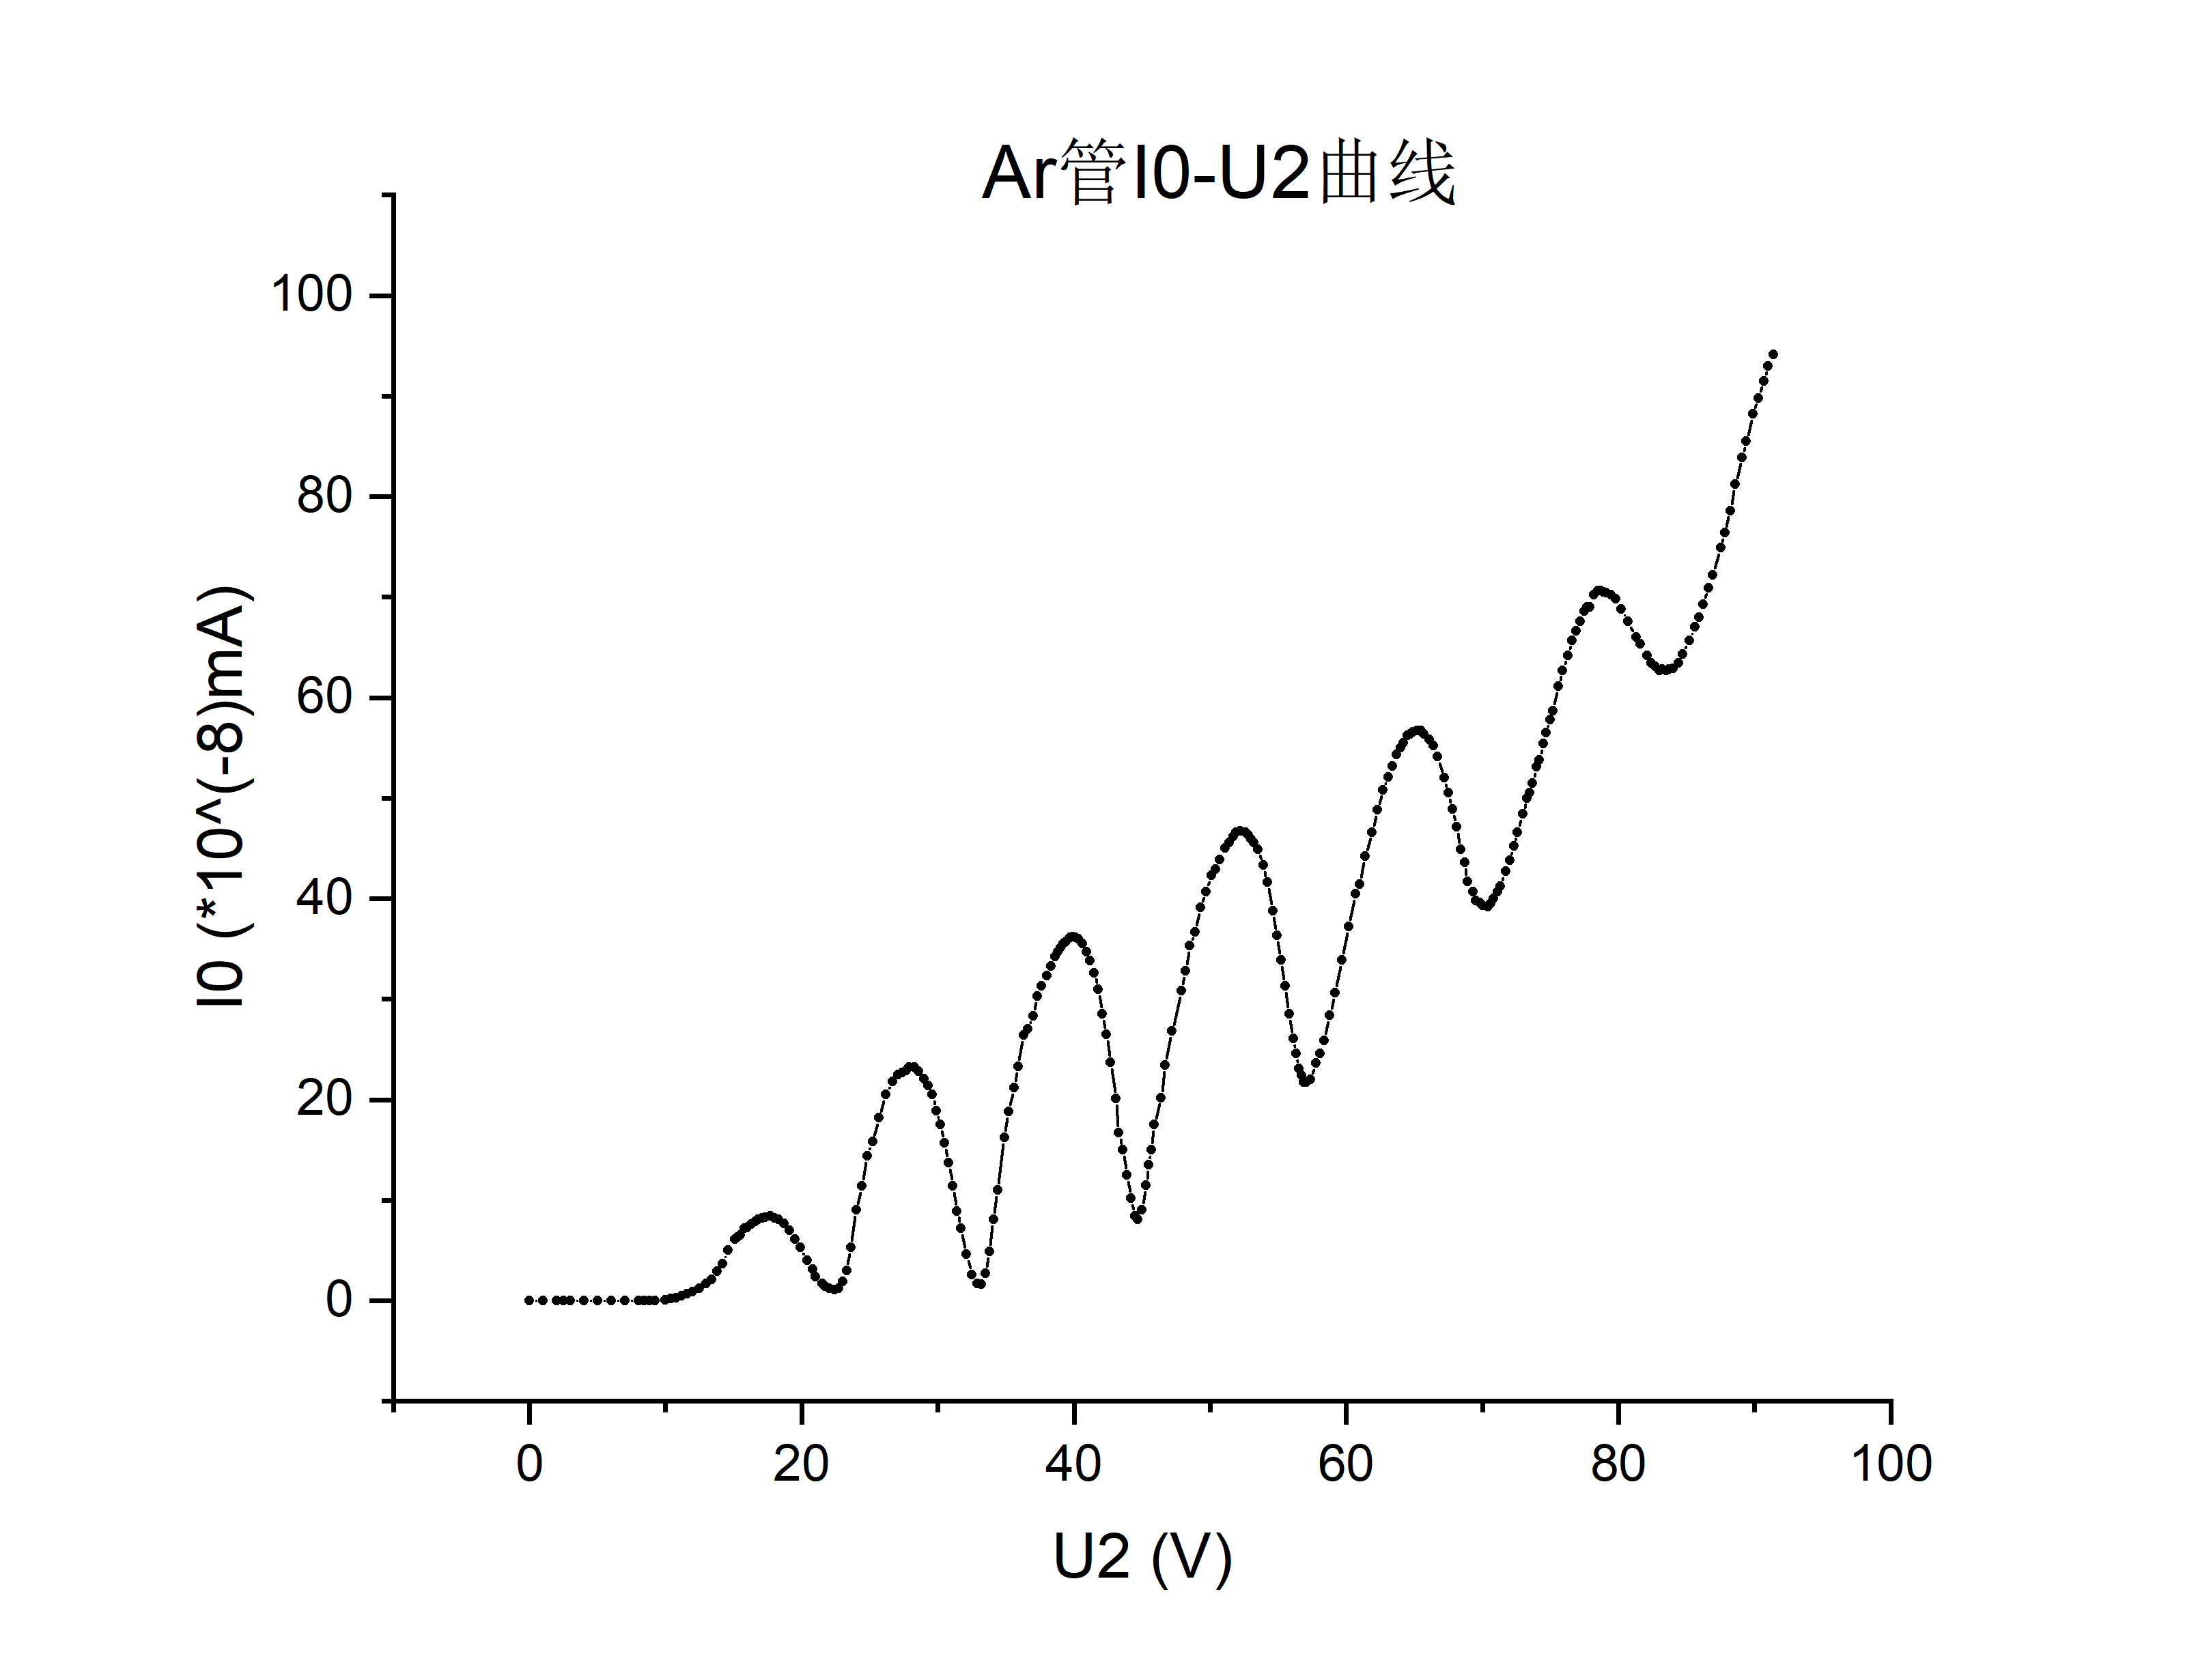
\includegraphics[width=0.8\textwidth]{Ar curve.jpg}
    \end{center}

    \subsection{Hg与Ar的第一激发电位}
    \subsubsection{Hg的第一激发电位}
    选取Hg管P极电压随加速电压曲线中的峰值扫描电压,如下表所示:

    \begin{center}
        \begin{tabular}{|c|c|c|c|c|c|c|}
            \hline
            x     & 1     & 2     & 3     & 4     & 5     & 6  \bigstrut\\
            \hline
            $U_0^{peak}(mV)$ & 5.2   & 9.8   & 14.6  & 19.3  & 24.2  & 29.4  \bigstrut\\
            \hline
        \end{tabular}%
    \end{center}

    理论上来说,峰值扫描电压应该都是第一激发电压的整数倍,因此,由于表中x是等间距分布的,用最小二乘法拟合,
    $U_2-x$曲线的斜率即可视为第一激发电压。拟合结果如下图:

    \begin{center}
        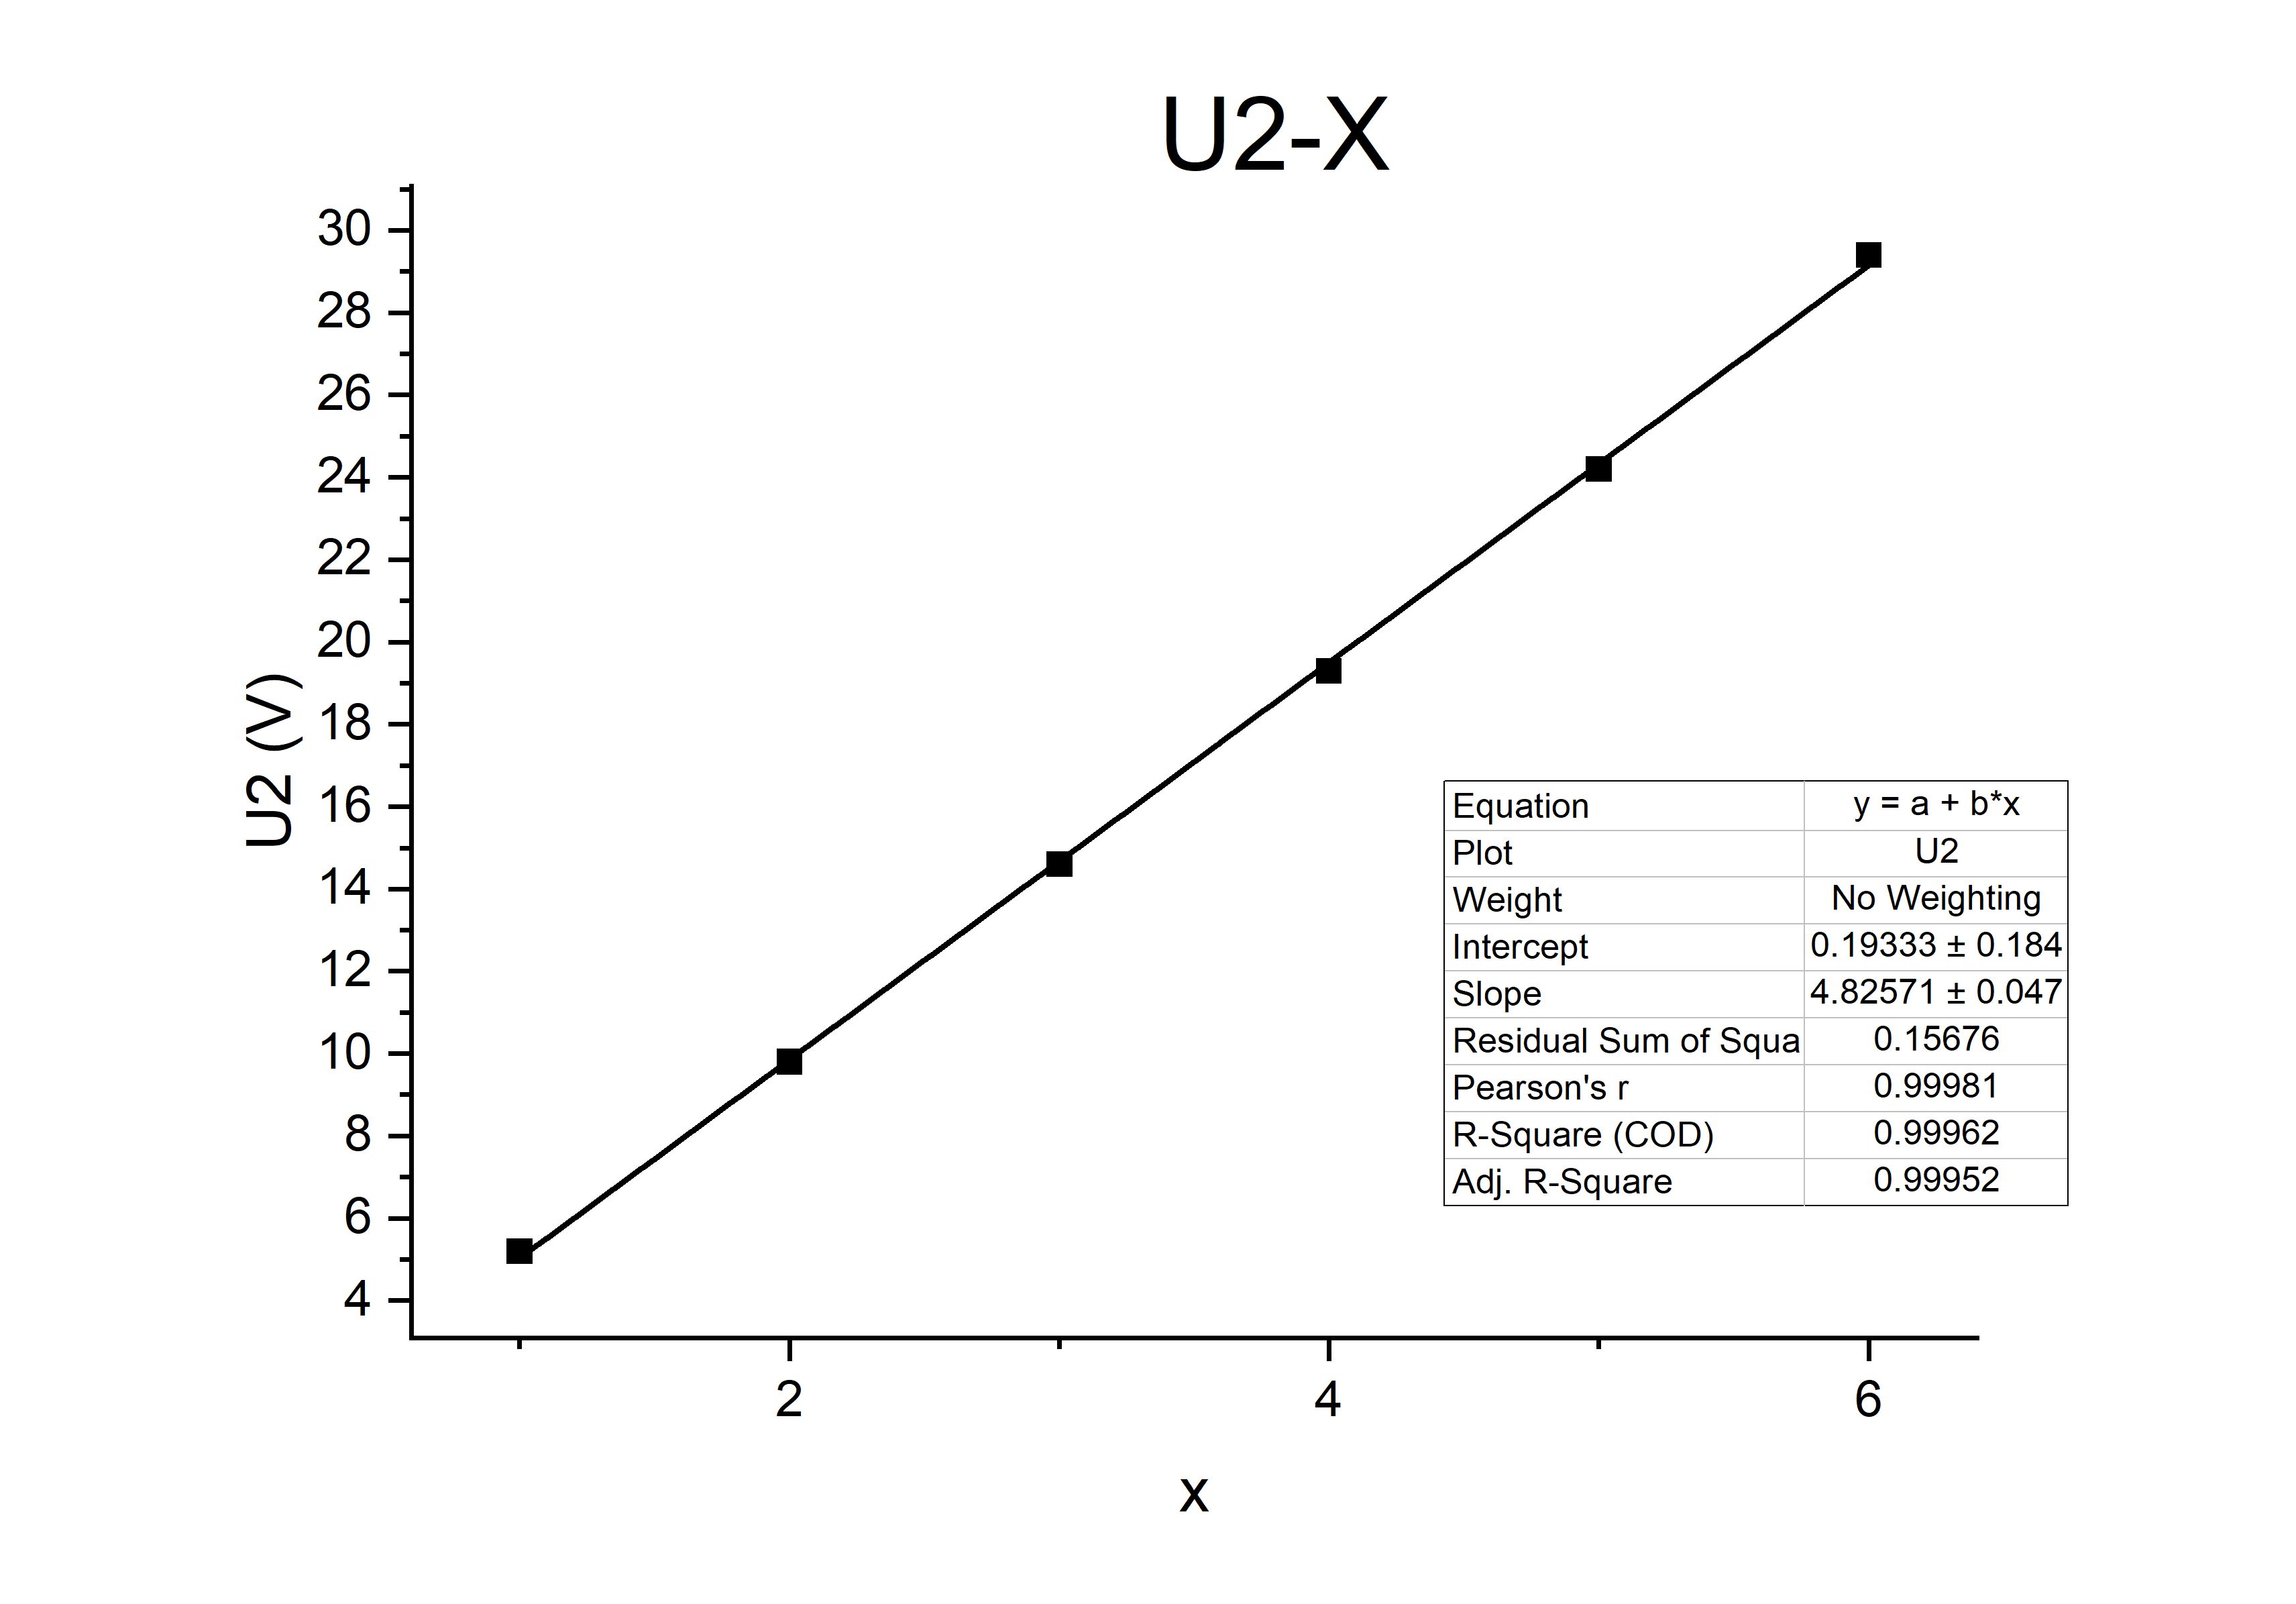
\includegraphics[width=\textwidth]{Hg activate.jpg}
    \end{center}

    从图中可知:
    $$U_1=k=4.82V,r=0.9998$$

    下面计算不确定度,其中,A类不确定度是来自拟合的不确定度,B类不确定度是来自允差的不确定度。实验中,在靠近峰值时,
    扫描电压的步长为$0.2V$或$0.1V$,保守起见,我们取允差为$0.2V$。
    $$\sigma_{U,A}=U_1\sqrt{\frac{1/r^2-1}{n-2}}=4.82\sqrt{\frac{1/0.9998^2-1}{6-2}}=0.048V$$
    $$\sigma_{U,B}=\frac{\sigma}{\sqrt{\sum_{i=1}^6 (x_i-\bar{x})^2}}=\frac{0.2/\sqrt{3}}{\sqrt{407.7}}=0.006V$$
    $$\sigma_{U}=\sqrt{(\sigma_{U,A})^2+(\sigma_{U,B})^2}=0.05V$$

    综上,Hg原子第一激发电压的测量结果为:
    $$U_1=(4.82\pm 0.05)V$$

    \subsubsection{Ar原子的第一激发电位}
    从氩管的P极电流随扫描电压变化曲线中截取峰值电流处的电压,如下表所示:

    \begin{center}
        \begin{tabular}{|c|c|c|c|c|c|c|}
            \hline
            x     & 1     & 2     & 3     & 4     & 5     & 6  \bigstrut\\
            \hline
            $U_2(V)$ & 17.7  & 28.3  & 39.9  & 52.2  & 65.2  & 78.5  \bigstrut\\
            \hline
        \end{tabular}%
    \end{center}

    同样用最小二乘法对数据进行处理,结果如下图所示:

    \begin{center}
        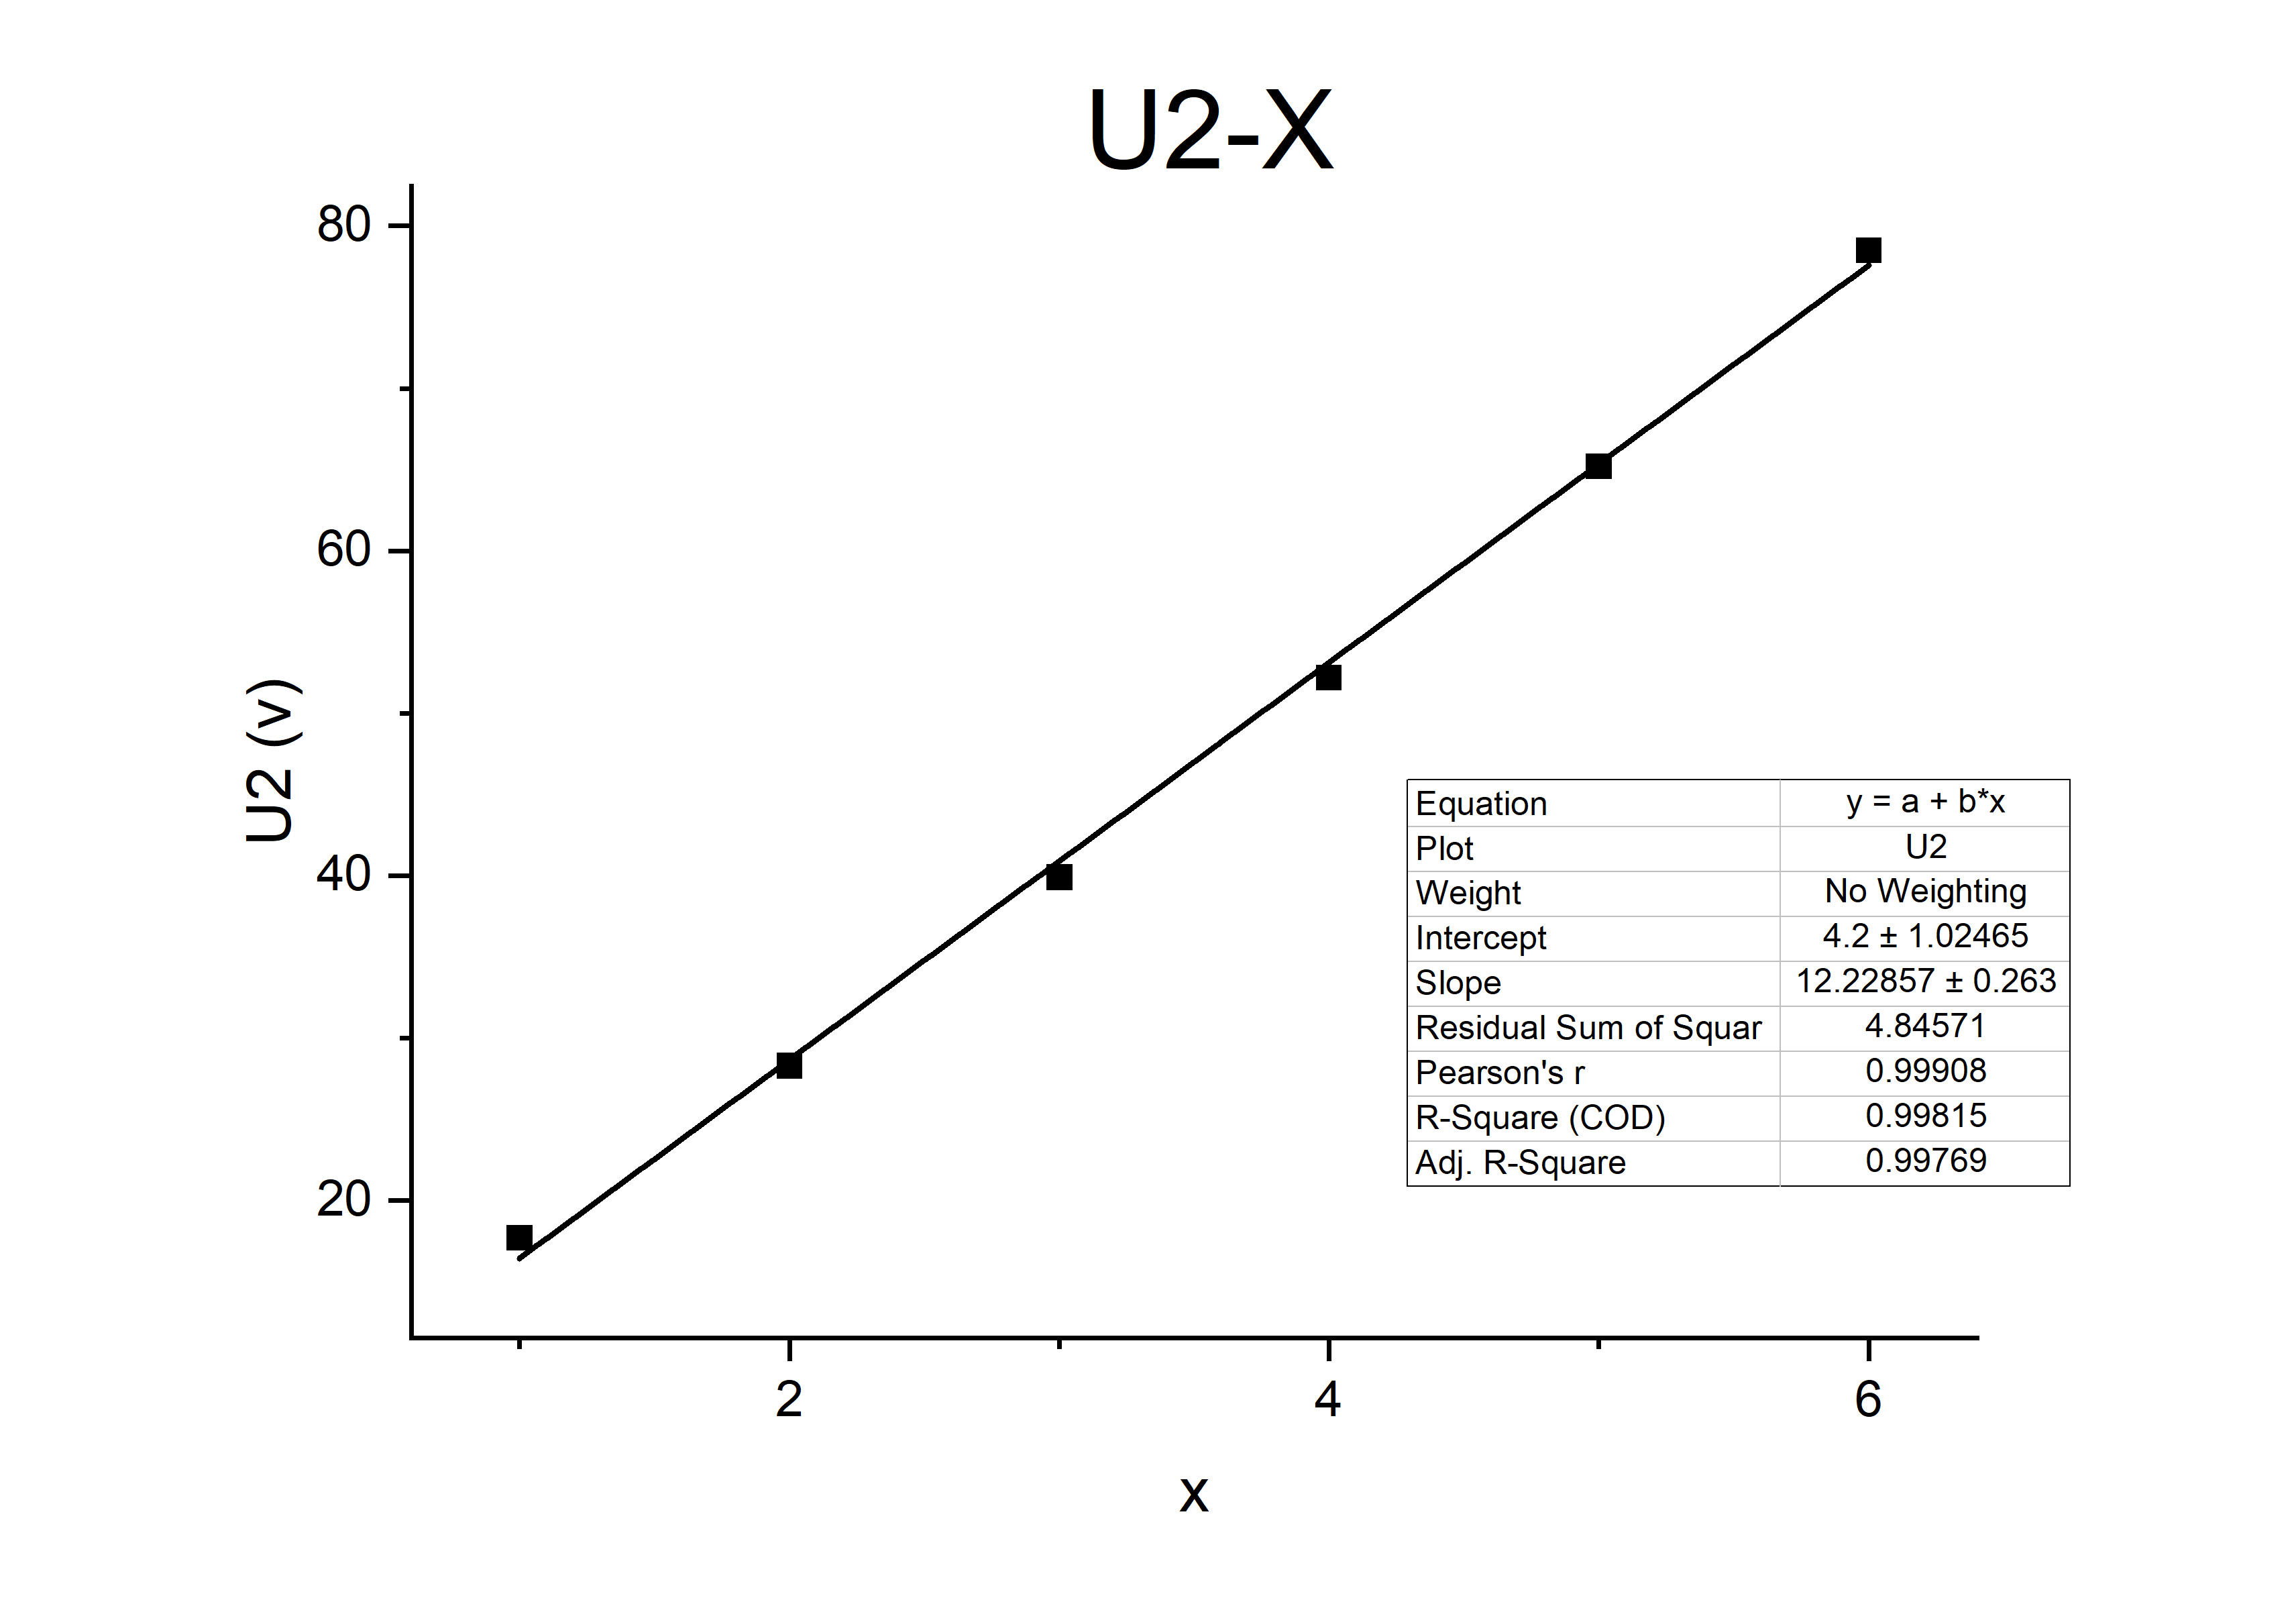
\includegraphics[width=0.8\textwidth]{Ar activate.jpg}
    \end{center}

    由拟合结果可知:
    $$U_1=12.23V,r=0.9991$$

    下面计算不确定度,实验中,在峰值附近扫描电压步长为$0.2V$或$0.3V$,保守起见取允差为$0.3V$
    $$\sigma_{U,A}=U_1\sqrt{\frac{1/r^2-1}{n-2}}=12.23\sqrt{\frac{1/0.9991^2-1}{6-2}}=0.26V$$
    $$\sigma_{U,B}=\frac{\sigma}{\sqrt{\sum_{i=1}^6 (x_i-\bar{x})^2}}=\frac{0.3/\sqrt{3}}{\sqrt{2609.1}}=0.003V$$
    $$\sigma_{U}=\sqrt{(\sigma_{U,A})^2+(\sigma_{U,B})^2}=0.26V$$

    综上,Ar原子第一激发电位的测量结果为:
    $$U_1=(12.23\pm0.26)V$$

    \subsection{改变减速电压$U_{g_2P}$后的测量结果}
    实验中,对汞管进行操作,在保证其加热温度和$U_{Kg_1}$不变的情况下,改变减速电压$U_{g_2P}$,对中间两个峰值附近进行扫描,
    研究减速电压对P极电流的影响。实验数据如下:

    $U_{Kg_1}=1.05V,U_{g_2P}=1.18V,\theta =175\degreesCelsius$

    \begin{center}
        \begin{tabular}{|c|c|c|c|c|c|c|c|c|c|c|c|}
            \hline
            $U_2(V)$ & 13.9  & 14.1  & 14.3  & 14.5  & 14.6  & 14.8  & 15.0  & 15.2  & 15.5  & 15.8  & 16.0  \bigstrut\\
            \hline
            $U_0(mV)$ & 98.3  & 119.7  & 133.5  & 150.1  & 156.9  & 158.9  & 132.5  & 83.4  & 44.6  & 24.2  & 16.0  \bigstrut\\
            \hline
        \end{tabular}%
    \end{center}

    续表

    \begin{center}
        \begin{tabular}{|c|c|c|c|c|c|c|c|c|c|c|c|}
            \hline
            $U_2(V)$ & 16.2  & 16.3  & 16.5  & 16.8  & 17.1  & 17.4  & 17.7  & 18.0  & 18.3  & 18.6  & 18.9  \bigstrut\\
            \hline
            $U_0(mV)$ & 19.4  & 20.5  & 22.6  & 31.8  & 44.0  & 56.8  & 72.6  & 95.7  & 124.1  & 157.9  & 190.1  \bigstrut\\
            \hline
        \end{tabular}%            
    \end{center}

    续表

    \begin{center}
        \begin{tabular}{|c|c|c|c|c|c|c|c|c|c|c|c|}
            \hline
            $U_2(V)$ & 19.1  & 19.3  & 19.4  & 19.5  & 19.6  & 19.8  & 20.1  & 20.4  & 20.6  & 20.8  & 21.0  \bigstrut\\
            \hline
            $U_0(mV)$ & 211.0  & 234.5  & 237.3  & 234.6  & 228.4  & 189.7  & 134.0  & 78.5  & 50.3  & 37.9  & 33.0  \bigstrut\\
            \hline
        \end{tabular}%
    \end{center}

    续表

    \begin{center}
        \begin{tabular}{|c|c|c|c|c|c|}
            \hline
            $U_2(V)$ & 21.2  & 21.3  & 21.5  & 21.6  & 21.9  \bigstrut\\
            \hline
            $U_0(mV)$ & 30.2  & 29.4  & 31.0  & 34.5  & 45.5  \bigstrut\\
            \hline
        \end{tabular}%
    \end{center}

    将减速电压改变前后的曲线绘制于同一张图中,其中红色曲线对应减速电压$U_{g_2P}=1.18V$,黑色曲线对应减速电压$U_{g_2P}=1.56V$

    \begin{center}
        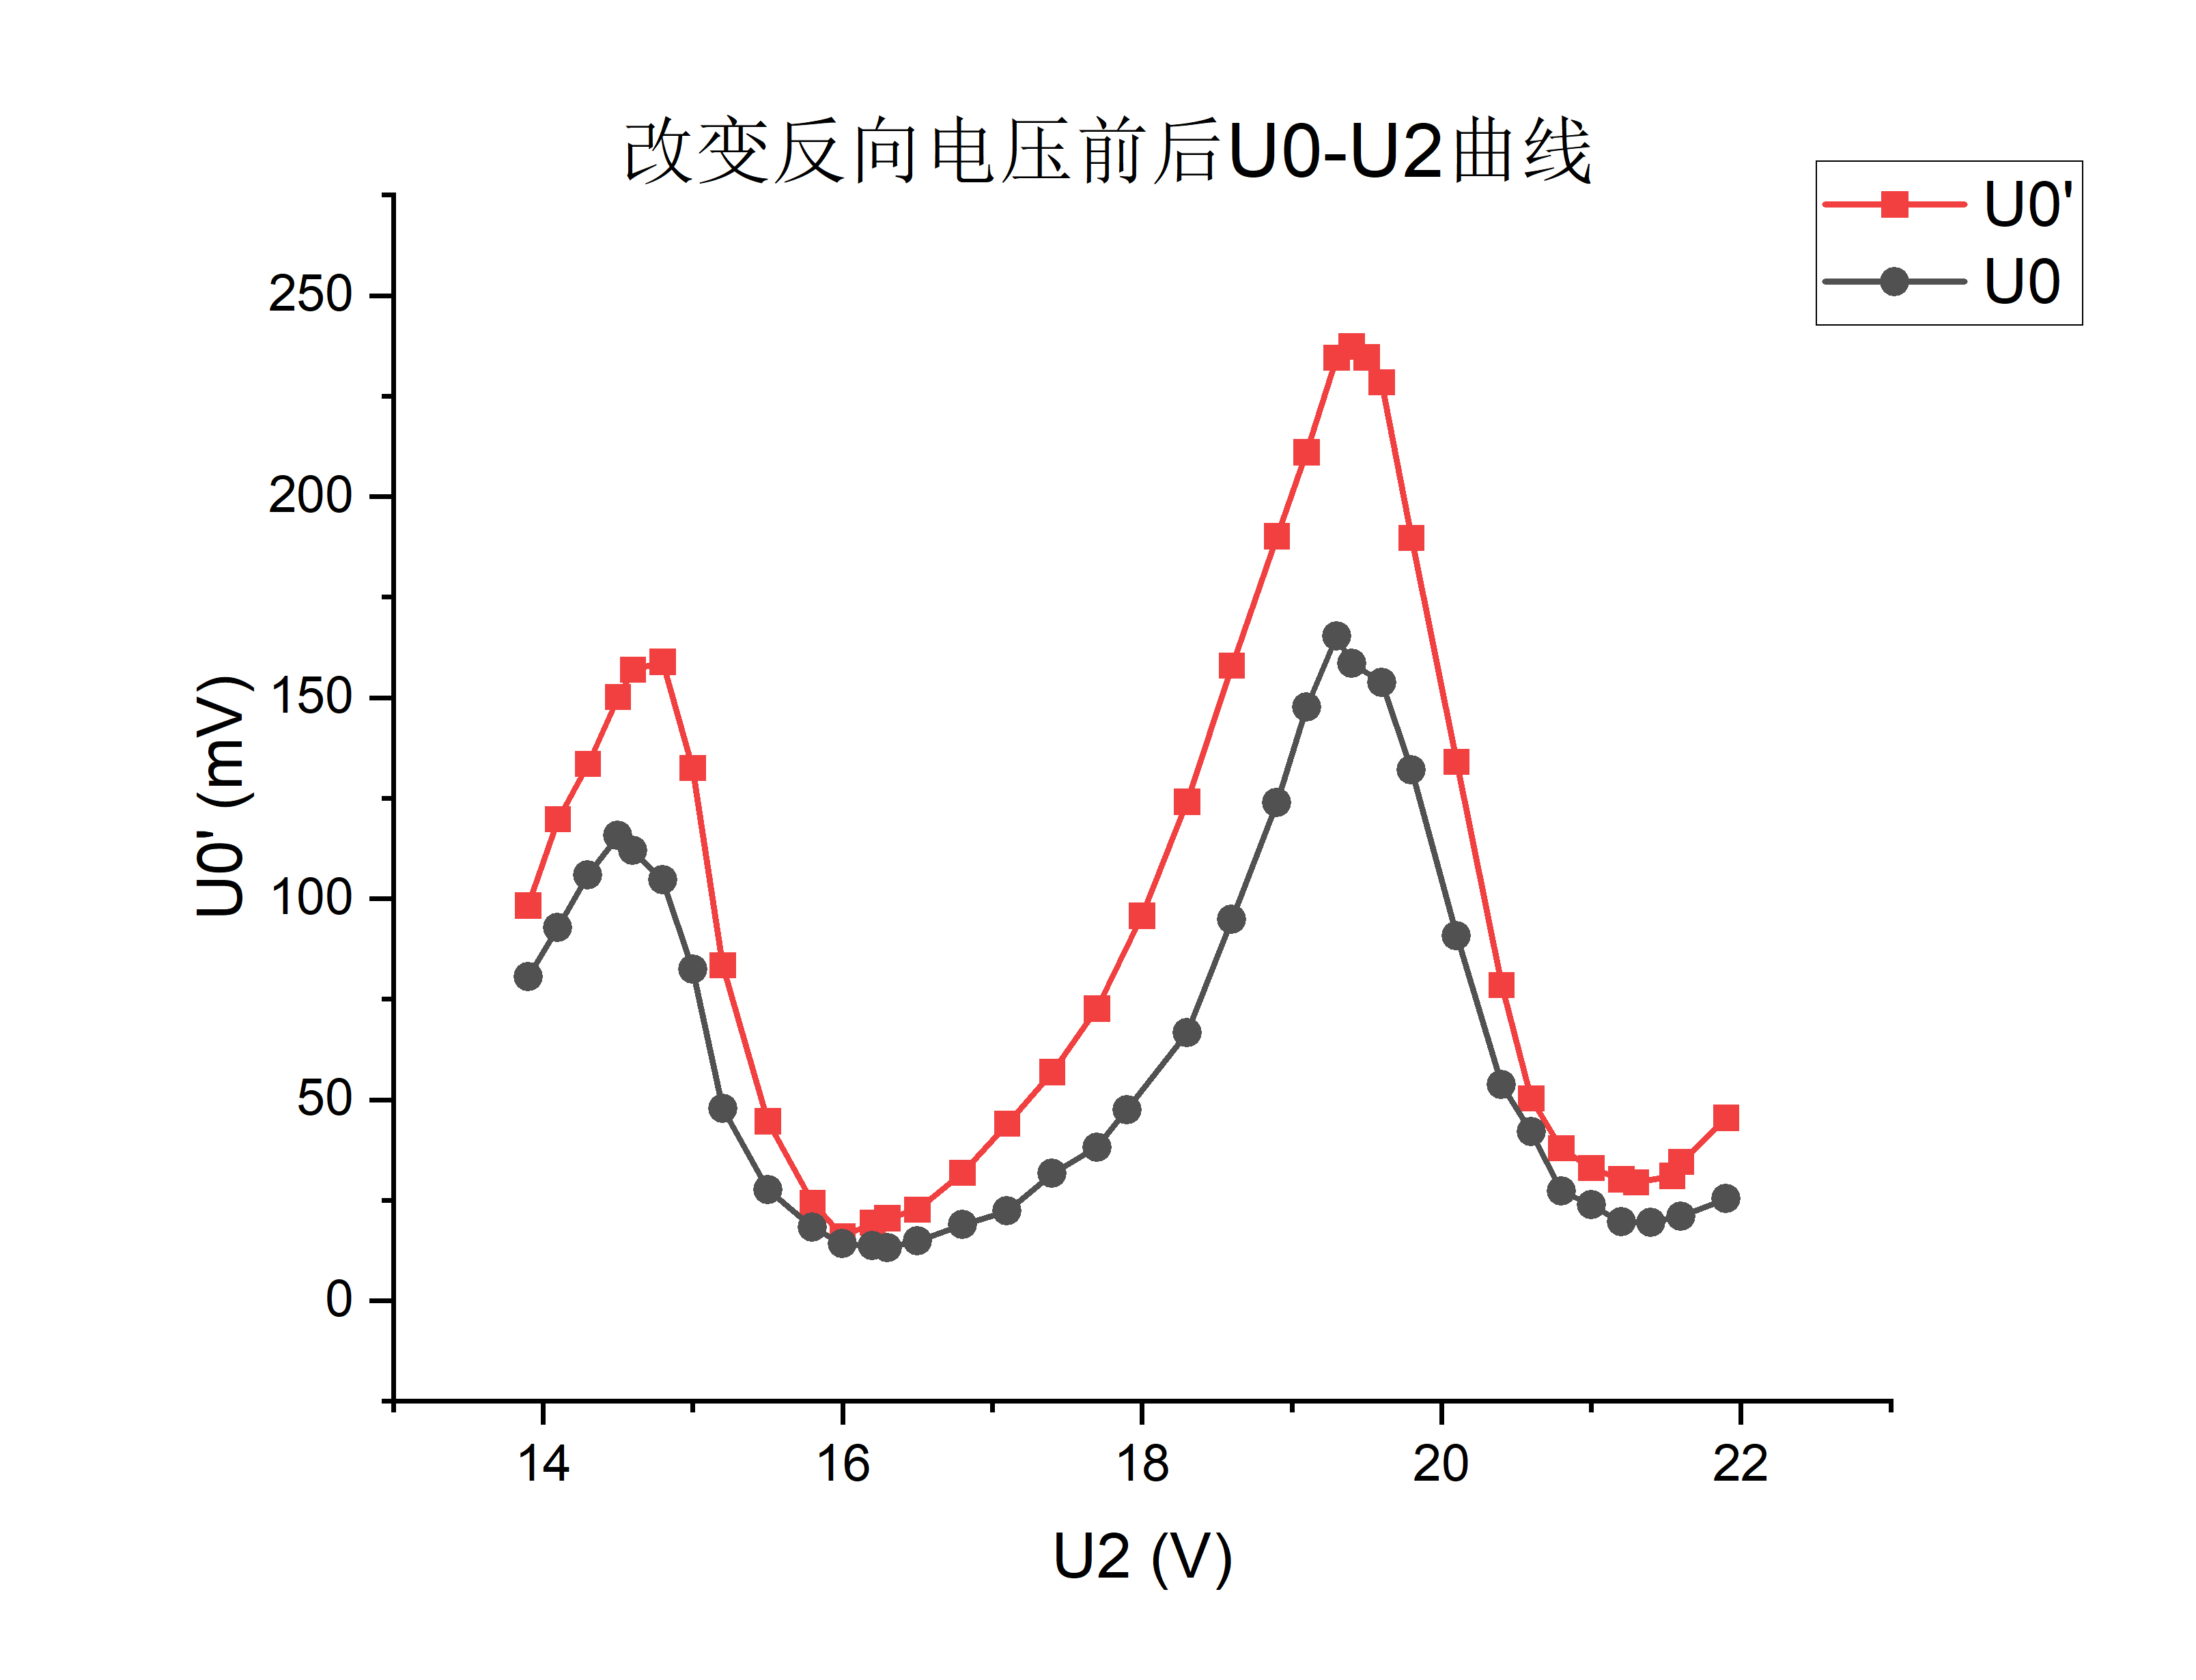
\includegraphics[width=0.8\textwidth]{reverse.jpg}
    \end{center}

    \section{思考题}
    \subsection{改变减速电压$U_{g_2P}$对曲线有何影响?}
    改变减速电压后的实验数据和实验曲线如section1.3中所示,从对比图中可以看出,改变减速电压前后,峰值和谷值电压
    对应的扫描电压基本不发生变化;但当减速电压减小,峰值电压和谷值电压均变大,其中峰值电压增大更明显。

    这是因为峰值电压和谷值电压对应的扫描电压只和F-H管中气体原子的激发态电压有关,与减速电压无关;
    而由于减速电压会起到拦截电子的作用,即经过加速电场后,动能低的原子不能到达P极,因此减小反向电压,能够使一些动能较低的、
    原本无法到达P极的电子到达P极,因此到达P极的电子数量增加,P极的电压也因此增加

    \section{分析与讨论}
    \subsection{实验中测得的各种曲线有什么主要特征?}
    Hg原子与Ar原子P极电压(流)随扫描电压的变化曲线,都是呈现周期性地上升-下降趋势,且周期大致为各原子的第一激发电压。
    峰值电压(流)出现在扫描电压为第一激发电压整数倍时附近,即当扫描电压达到第一激发电压整数倍时P极电压(流)会突降,
    降到谷底后再缓慢回升,然后再次突降。

    此外,两根曲线中,Hg原子的曲线峰处较为尖锐,谷处较为平滑,而Ar曲线则相反,峰处较为平滑,谷处较为尖锐。Hg和Ar峰谷值对应的扫描电压不同。

    观察两根曲线还能发现,随着扫描电压的增大,峰值和谷值电压(流)都呈现增大的趋势,其中峰值比谷值增大更明显,Ar管比Hg管峰谷值增大更明显。

    为了测量第一激发电压,我们作了峰值电压(流)对应扫描电压的曲线,Hg管与Ar管的曲线都非常接近直线,说明峰值电压(流)对应扫描电压
    基本上是等间距分布的,差即为第一激发电压。但Hg的曲线中,y轴截距几乎为0;而Ar曲线中,y轴截距有12V左右。

    以上这些曲线特征,Hg的曲线和Ar的曲线的一些共性,如周期性上升下降,来自于原子中电子共同的量子化轨道和能级结构;而两者的不同,
    如曲线的增大趋势,一方面来源于Hg原子和Ar原子更进一步的特征,另一方面也与两管的其他实验条件有关。

    \subsection{测量第一激发电位时误差的主要来源}
    主要来源于对峰值/谷值电压(流)判断的不准确性。
    
    对于Hg管来说,由于P极电压的数字跳动很大,很难判断P极电压到底是多少,且在峰谷值附近,电压的变化趋势较缓,
    更难以判断到底哪个扫描电压对应的P极电压使峰值/谷值。对于Ar管来说,由于其P极电流随时间推移会发生变化,
    也很难判断是否已经达到峰谷值。

    此外,扫描电压的调节是有一定步长的,虽然在峰谷附近减小了步长,但仍然有0.2V或0.3V的步长,因此峰谷值实际上只是出现
    在这0.2V或0.3V的区间内某一位置,并不能保证精准地对应于P极电压(流)最大的那个扫描电压。

    \section{收获与感想}
    该实验可能是本学期做的所有实验中数据量最大的一个,但抛开数据量,本实验加深了我们对于原子的能级结构的认识,同时通过对
    管中电子具体行为的分析,可以更好地了解电磁学相关知识。在大数据量前提下对实验的操作和对数据的处理也提升了我们的实验技能。

\end{document}